\documentclass[sublist]{fei}
\usepackage[utf8]{inputenc}

\author{André de Souza Mendes}
\title{Articulated vehicle model}
%\subtitulo{subtítulo}
%\cidade{cidade}
\instituicao{Vehicle Dynamics - Lateral}

\makeindex
\makeglossaries

\begin{document}

\maketitle

% \begin{folhaderosto}
% Dissertação de Mestrado apresentada ao Centro Universitário da FEI para obtenção do título de Mestre em Engenharia Mecânica, orientado pelo Prof. Dr. Agenor de Toledo Fleury.
% \end{folhaderosto}

% \fichacatalografica						% procura o arquivo "ficha.pdf"
% \folhadeaprovacao						% procura o arquivo "ata.pdf"

% \dedicatoria{À minha família.}

% \begin{agradecimentos}
% Obrigado
% \end{agradecimentos}

% \epigrafe{Science is more than a body of knowledge, it's a way of thinking. A way of skeptically interrogating the universe with a fine understanding of human fallibility.}{Carl Sagan}

% \begin{resumo}
% resumo
% \palavraschave{Dinâmica veicular. Veículos articulados. Análise de estabilidade. Trajetórias de fase. Expoentes de Lyapunov.}
% \end{resumo}

% \begin{abstract}
% abstract
% \keywords{Vehicle dynamics. Articulated vehicles. Stability analysis. Phase trajectories. Lyapunov exponents.}
% \end{abstract}

% {
% 	\pagestyle{empty}
% 	\listoffigures
% 	\listoftables
% %	\listofalgorithms
%     \printglossaries
%     % \glsaddall
%     \tableofcontents
% }




\section{Usando Lagrange}

O modelo físico do carro é ilustrado na figura \ref{modelSimple}. A base \( \{ {\rm O} {\bf i} {\bf j} {\bf k} \}\) é fixa no referencial inercial. A base \( \{ {\rm T} {\bf t}_x {\bf t}_y {\bf t}_z \}\) é solidária ao veículo. A base \( \{ {\rm F} {\bf e}_x {\bf e}_y {\bf e}_z \}\) é solidária ao eixo dianteiro. O ponto \({\rm T}\) localiza o centro de massa do veículo. \({\rm F}\) e \({\rm R}\) localizam os eixos dianteiro e traseiro, respectivamente. O ponto \({\rm O}\) é a origem do sistema e se encontra fixo no referencial inercial. A distância \(a\) separa os pontos \({\rm F}\) e \({\rm T}\) e a distância \(b\) separa os pontos \({\rm T}\) e \({\rm R}\).
a
As coordenadas generalizadas são dadas por

\begin{subequations}
\begin{equation}
    q_1 = x
\end{equation}
\begin{equation}
    q_2 = y
\end{equation}
\begin{equation}
    q_3 = \psi,
\end{equation}
\end{subequations}
onde \(x\) e \(y\) são as coordenadas longitudinais do centro de massa do carro nas direções horizontal e vertical, respectivamente. \(\psi\) é o ângulo de orientação absoluta do veículo.

\begin{figure}
    \begin{center}
    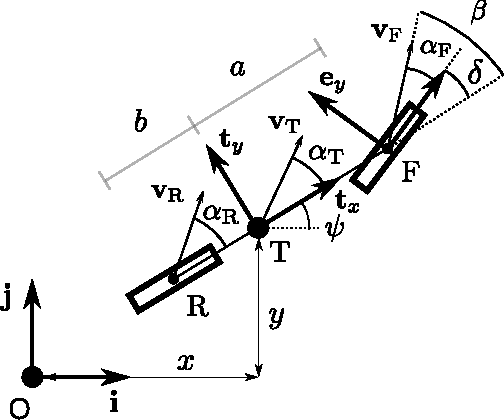
\includegraphics{../illustrations/modelSimple.pdf}
    \caption{Single track bicycle model.} \label{modelSimple}
    \end{center}
\end{figure}

O vetor posição do centro de massa em relação ao ponto \(O\) é

\begin{equation} \label{positionTractor}
    {\bf p}_{{\rm T}/{\rm O}} = x {\bf i} + y {\bf j}.
\end{equation}

Derivando a equação \eqref{positionTractor} em relação ao tempo temos

\begin{equation}
    {\bf v}_{\rm T} = \dot{x} {\bf i} + \dot{y} {\bf j}.
\end{equation}

A energia cinética do sistema é

\begin{equation}
    T = \frac{1}{2} m_{T} {\bf v}_{\rm T} \cdot {\bf v}_{\rm T} + \frac{1}{2} I_{T} \dot{\psi}^2.
\end{equation}

Ou ainda,

\begin{equation}
    T = \frac{1}{2} m_{T} \left( \dot{x}^2 + \dot{y}^2 \right) + \frac{1}{2} I_{T} \dot{\psi}^2.
\end{equation}

A velocidade no eixo dianteiro é dada por

\begin{equation}
    {\bf v}_{\rm F} = {\bf v}_{\rm T} + {\bf r} \wedge {\bf r}_{{\rm F}/{\rm T}},
\end{equation}
onde \({\bf r}_{{\rm F}/{\rm T}}\) é o vetor posição do ponto \({\rm F}\) em relação ao ponto \({\rm T}\). Logo,

\begin{equation} \label{velocityVectorFront}
    {\bf v}_{\rm F} = \left( \dot{x} - a \dot{\psi} \sin \psi \right) {\bf i} + \left( \dot{y} + a \dot{\psi} \cos \psi \right) {\bf j}.
\end{equation}

A velocidade no eixo traseiro é

\begin{equation}
    {\bf v}_{\rm R} = {\bf v}_{\rm T} + {\bf r} \wedge {\bf r}_{{\rm R}/{\rm T}},
\end{equation}
onde \({\bf r}_{{\rm R}/{\rm T}}\) é o vetor posição do ponto \({\rm R}\) em relação ao ponto \({\rm T}\). Logo,

\begin{equation} \label{velocityVectorRear}
    {\bf v}_{\rm R} = \left( \dot{x} + b \dot{\psi} \sin \psi \right) {\bf i} + \left( \dot{y} -b \dot{\psi} \cos \psi \right) {\bf j}
\end{equation}

Utilizando as equações \eqref{velocityVectorFront} e \eqref{velocityVectorRear}, os ângulos de deriva podem ser escritos como

\begin{subequations}
\begin{equation} \label{slipAngleFront}
    \alpha_{\rm F} = \arctan \left( \frac{\dot{y} + a \dot{\psi} \cos \psi}{ \dot{x} - a \dot{\psi} \sin \psi} \right) - \left( \delta + \psi \right)
\end{equation}
\begin{equation} \label{slipAngleRear}
    \alpha_{\rm R} = \arctan \left( \frac{\dot{y} - b \dot{\psi} \cos \psi}{ \dot{x} + b \dot{\psi} \sin \psi} \right) - \psi
\end{equation}
\end{subequations}

A força do eixo dianteiro é dadas por

\begin{equation}
    {\bf F}_{\rm F} = F_{x,{\rm F}} {\bf e}_x + F_{y,{\rm F}} {\bf e}_x,
\end{equation}
que pode ser escrita como

\begin{equation} \label{ForceAtFront}
    {\bf F}_{\rm F} = \left[ F_{x,{\rm F}} \cos \left( \psi + \delta \right) - F_{y,{\rm F}} \sin \left( \psi + \delta \right) \right] {\bf i} + \left[ F_{x,{\rm F}} \sin \left( \psi + \delta \right) + F_{y,{\rm F}} \cos \left( \psi + \delta \right) \right] {\bf j}.
\end{equation}

A força no eixo traseiro é

\begin{equation}
    {\bf F}_{\rm R} = F_{x,{\rm R}} {\bf t}_x + F_{y,{\rm R}} {\bf t}_y
\end{equation}
ou

\begin{equation} \label{ForceAtRear}
    {\bf F}_{\rm R} = \left[ F_{x,{\rm R}} \cos \psi - F_{y,{\rm R}} \sin \psi \right] {\bf i} + \left[ F_{x,{\rm R}} \sin \psi + F_{y,{\rm R}} \cos \psi \right] {\bf j}.
\end{equation}

As forças generalizadas são

\begin{equation}
    Q_k = \sum_{j = 1} ^p {\bf F}_j \cdot \frac{\partial {\bf p}_j}{\partial q_k}
\end{equation}

No modelo

\begin{subequations} \label{generalizedForces}
\begin{equation}
    Q_1 = {\bf F}_{\rm F} \cdot \frac{\partial {\bf p}_{{\rm F}/{\rm O}}}{\partial q_1} + {\bf F}_{\rm R} \cdot \frac{\partial {\bf p}_{{\rm R}/{\rm O}}}{\partial q_1}
\end{equation}
\begin{equation}
    Q_2 = {\bf F}_{\rm F} \cdot \frac{\partial {\bf p}_{{\rm F}/{\rm O}}}{\partial q_2} + {\bf F}_{\rm R} \cdot \frac{\partial {\bf p}_{{\rm R}/{\rm O}}}{\partial q_2}
\end{equation}
\begin{equation}
    Q_3 = {\bf F}_{\rm F} \cdot \frac{\partial {\bf p}_{{\rm F}/{\rm O}}}{\partial q_3} + {\bf F}_{\rm R} \cdot \frac{\partial {\bf p}_{{\rm R}/{\rm O}}}{\partial q_3},
\end{equation}
\end{subequations}
onde

\begin{subequations} \label{termGenFor1}
\begin{equation}
    \frac{\partial {\bf p}_{{\rm F}/{\rm O}}}{\partial q_1} = \frac{\partial {\bf p}_{{\rm F}/{\rm O}}}{\partial x} = {\bf i}
\end{equation}
\begin{equation}
    \frac{\partial {\bf p}_{{\rm F}/{\rm O}}}{\partial q_2} = \frac{\partial {\bf p}_{{\rm F}/{\rm O}}}{\partial y} = {\bf j}
\end{equation}
\begin{equation}
    \frac{\partial {\bf p}_{{\rm F}/{\rm O}}}{\partial q_3} = \frac{\partial {\bf p}_{{\rm F}/{\rm O}}}{\partial \psi} = - a \sin \psi {\bf i} + a \cos \psi {\bf j}
\end{equation}
\end{subequations}
e

\begin{subequations} \label{termGenFor2}
\begin{equation}
    \frac{\partial {\bf p}_{{\rm R}/{\rm O}}}{\partial q_1} = \frac{\partial {\bf p}_{{\rm R}/{\rm O}}}{\partial x} = {\bf i}
\end{equation}
\begin{equation}
    \frac{\partial {\bf p}_{{\rm R}/{\rm O}}}{\partial q_2} = \frac{\partial {\bf p}_{{\rm R}/{\rm O}}}{\partial y} = {\bf j}
\end{equation}
\begin{equation}
    \frac{\partial {\bf p}_{{\rm R}/{\rm O}}}{\partial q_3} = \frac{\partial {\bf p}_{{\rm R}/{\rm O}}}{\partial \psi} = b \sin \psi {\bf i} - b \cos \psi {\bf j}
\end{equation}
\end{subequations}

Substituindo as equações \eqref{ForceAtFront}, \eqref{ForceAtRear}, \eqref{termGenFor1} e \eqref{termGenFor2} nas equações \eqref{generalizedForces} temos

\begin{subequations}
\begin{equation}
    Q_1 = F_{x,{\rm F}} \cos \left( \psi + \delta \right) + F_{x,{\rm R}} \cos \psi - F_{y,{\rm F}} \sin \left( \psi + \delta \right) - F_{y,{\rm R}} \sin \psi
\end{equation}
\begin{equation}
    Q_2 = F_{x,{\rm F}} \sin \left( \psi + \delta \right)+ F_{x,{\rm R}} \sin \psi + F_{y,{\rm F}} \cos \left( \psi + \delta \right) + F_{y,{\rm R}} \cos \psi
\end{equation}
\begin{equation}
    Q_3 =  F_{x,{\rm F}} a \sin \delta  + F_{y,{\rm F}} a \cos \delta - F_{y,{\rm R}} b.
\end{equation}
\end{subequations}

A formulação de Lagrange é dada por

\begin{equation} \label{lagrange}
    \frac{d}{dt} \left( \frac{\partial T}{\partial \dot{q}_k} \right) - \frac{\partial T}{\partial q_k} = Q_k.
\end{equation}

Para as três coordenadas generalizadas do sistema

\begin{subequations} \label{lagrangeSecond}
\begin{equation}
    \frac{\partial T}{\partial q_1} = \frac{\partial T}{\partial x} = 0
\end{equation}
\begin{equation}
    \frac{\partial T}{\partial q_2} = \frac{\partial T}{\partial y} = 0
\end{equation}
\begin{equation}
    \frac{\partial T}{\partial q_3} = \frac{\partial T}{\partial \psi} = 0,
\end{equation}
\end{subequations}

\begin{subequations}
\begin{equation}
    \frac{\partial T}{\partial \dot{q}_1} = \frac{\partial T}{\partial \dot{x}} = m_{T} \dot{x}
\end{equation}
\begin{equation}
    \frac{\partial T}{\partial \dot{q}_2} = \frac{\partial T}{\partial \dot{y}} = m_{T} \dot{y}
\end{equation}
\begin{equation}
    \frac{\partial T}{\partial \dot{q}_3} = \frac{\partial T}{\partial \dot{\psi}} = I_{T} \dot{\psi},
\end{equation}
\end{subequations}

\begin{subequations} \label{lagrangeFirst}
\begin{equation}
    \frac{d}{dt} \left( \frac{\partial T}{\partial \dot{q}_1} \right) = \frac{d}{dt} \left( \frac{\partial T}{\partial \dot{x}} \right) = m_{T} \ddot{x}
\end{equation}
\begin{equation}
    \frac{d}{dt} \left( \frac{\partial T}{\partial \dot{q}_2} \right) = \frac{d}{dt} \left( \frac{\partial T}{\partial \dot{y}} \right) = m_{T} \ddot{y}
\end{equation}
\begin{equation}
    \frac{d}{dt} \left( \frac{\partial T}{\partial \dot{q}_3} \right) = \frac{d}{dt} \left( \frac{\partial T}{\partial \dot{\psi}} \right) = I_{T} \ddot{\psi}.
\end{equation}
\end{subequations}

Substituindo \eqref{lagrangeFirst} e \eqref{lagrangeSecond} em \eqref{lagrange} temos as equações de movimento

\begin{subequations}
\begin{equation}
    m_{T} \ddot{x} = F_{x,{\rm F}} \cos \left( \psi + \delta \right) + F_{x,{\rm R}} \cos \psi - F_{y,{\rm F}} \sin \left( \psi + \delta \right) - F_{y,{\rm R}} \sin \psi
\end{equation}
\begin{equation}
    m_{T} \ddot{y} = F_{x,{\rm F}} \sin \left( \psi + \delta \right)+ F_{x,{\rm R}} \sin \psi + F_{y,{\rm F}} \cos \left( \psi + \delta \right) + F_{y,{\rm R}} \cos \psi
\end{equation}
\begin{equation}
    I_{T} \ddot{\psi} = F_{x,{\rm F}} a \sin \delta  + F_{y,{\rm F}} a \cos \delta - F_{y,{\rm R}} b,
\end{equation}
\end{subequations}
ou seja,

\begin{subequations} \label{equationOfMotion}
\begin{equation}
    \ddot{x} = \frac{F_{x,{\rm F}} \cos \left( \psi + \delta \right) + F_{x,{\rm R}} \cos \psi - F_{y,{\rm F}} \sin \left( \psi + \delta \right) - F_{y,{\rm R}} \sin \psi}{m_{T}}
\end{equation}
\begin{equation}
    \ddot{y} = \frac{F_{x,{\rm F}} \sin \left( \psi + \delta \right)+ F_{x,{\rm R}} \sin \psi + F_{y,{\rm F}} \cos \left( \psi + \delta \right) + F_{y,{\rm R}} \cos \psi}{m_{T}}
\end{equation}
\begin{equation}
    \ddot{\psi} = \frac{F_{x,{\rm F}} a \sin \delta  + F_{y,{\rm F}} a \cos \delta - F_{y,{\rm R}} b}{I_{T}}.
\end{equation}
\end{subequations}

Os vetores de estado podem ser escolhidos como

\begin{subequations}
\begin{equation}
    {\rm z}_1 = x
\end{equation}
\begin{equation}
    {\rm z}_2 = y
\end{equation}
\begin{equation}
    {\rm z}_3 = \psi
\end{equation}
\begin{equation}
    {\rm z}_4 = \dot{x}
\end{equation}
\begin{equation}
    {\rm z}_5 = \dot{y}
\end{equation}
\begin{equation}
    {\rm z}_6 = \dot{\psi}
\end{equation}
\end{subequations}

Logo, as equações de estado são

\begin{subequations}
\begin{equation}
    \dot{{\rm z}}_1 = {\rm z}_4
\end{equation}
\begin{equation}
    \dot{{\rm z}}_2 = {\rm z}_5
\end{equation}
\begin{equation}
    \dot{{\rm z}}_3 = {\rm z}_6
\end{equation}
\begin{equation}
    \dot{{\rm z}}_4 = \frac{F_{x,{\rm F}} \cos \left( {\rm z}_3 + \delta \right) + F_{x,{\rm R}} \cos {\rm z}_3 - F_{y,{\rm F}} \sin \left( {\rm z}_3 + \delta \right) - F_{y,{\rm R}} \sin {\rm z}_3}{m_{T}}
\end{equation}
\begin{equation}
    \dot{{\rm z}}_5 = \frac{F_{x,{\rm F}} \sin \left( {\rm z}_3 + \delta \right)+ F_{x,{\rm R}} \sin {\rm z}_3 + F_{y,{\rm F}} \cos \left( {\rm z}_3 + \delta \right) + F_{y,{\rm R}} \cos {\rm z}_3}{m_{T}}
\end{equation}
\begin{equation}
    \dot{{\rm z}}_6 = \frac{F_{x,{\rm F}} a \sin \delta  + F_{y,{\rm F}} a \cos \delta - F_{y,{\rm R}} b}{I_{T}}
\end{equation}
\end{subequations}

Com os ângulos de deriva, a partir das equações \eqref{slipAngleFront} e \eqref{slipAngleRear},

\begin{equation}
    \alpha_{\rm F} = \arctan \left( \frac{{\rm z}_5 + a {\rm z}_6 \cos {\rm z}_3}{ {\rm z}_4 - a {\rm z}_6 \sin {\rm z}_3} \right) - \left( \delta + {\rm z}_3 \right)
\end{equation}

\begin{equation}
    \alpha_{\rm R} = \arctan \left( \frac{{\rm z}_5 - b {\rm z}_6 \cos {\rm z}_3}{ {\rm z}_4 + b {\rm z}_6 \sin {\rm z}_3} \right) - {\rm z}_3
\end{equation}

\section{Substituição dos estados}

Em muitas ocasiões é conveniente fazer a substituição dos estados \(\dot{x}\) e \(\dot{y}\) por \(v_{\rm T}\) e \(\alpha_{\rm T}\). A relação entre estes pares de estados é

\begin{subequations} \label{stateSubstitution}
\begin{equation}
    \dot{x} = v_{\rm T} \cos \left( \psi + \alpha_{\rm T} \right)
\end{equation}
\begin{equation}
    \dot{y} = v_{\rm T} \sin \left( \psi + \alpha_{\rm T} \right).
\end{equation}
\end{subequations}

Derivando em relação ao tempo a equação \eqref{stateSubstitution} temos

\begin{subequations} \label{stateDiffSubstitution}
\begin{equation}
    \ddot{x} = \dot{v}_{\rm T} \cos \left( \psi + \alpha_{\rm T} \right) - v_{\rm T} \left( \dot{\psi} + \dot{\alpha}_{\rm T} \right) \sin \left( \psi + \alpha_{\rm T} \right)
\end{equation}
\begin{equation}
    \ddot{y} = \dot{v}_{\rm T} \sin \left( \psi + \alpha_{\rm T} \right) + v_{\rm T} \left( \dot{\psi} + \dot{\alpha}_{\rm T} \right) \cos \left( \psi + \alpha_{\rm T} \right).
\end{equation}
\end{subequations}

Substituindo as equações \eqref{stateDiffSubstitution} nas equações \eqref{equationOfMotion}

\begin{subequations}
\begin{equation}
    \dot{v}_{\rm T} \cos \left( \psi + \alpha_{\rm T} \right) - v_{\rm T} \left( \dot{\psi} + \dot{\alpha}_{\rm T} \right) \sin \left( \psi + \alpha_{\rm T} \right) = \frac{F_{x,{\rm F}} \cos \left( \psi + \delta \right) + F_{x,{\rm R}} \cos \psi - F_{y,{\rm F}} \sin \left( \psi + \delta \right) - F_{y,{\rm R}} \sin \psi}{m_{T}}
\end{equation}
\begin{equation}
    \dot{v}_{\rm T} \sin \left( \psi + \alpha_{\rm T} \right) + v_{\rm T} \left( \dot{\psi} + \dot{\alpha}_{\rm T} \right) \cos \left( \psi + \alpha_{\rm T} \right) = \frac{F_{x,{\rm F}} \sin \left( \psi + \delta \right)+ F_{x,{\rm R}} \sin \psi + F_{y,{\rm F}} \cos \left( \psi + \delta \right) + F_{y,{\rm R}} \cos \psi}{m_{T}}
\end{equation}
\begin{equation}
    \ddot{\psi} = \frac{F_{x,{\rm F}} a \sin \delta  + F_{y,{\rm F}} a \cos \delta - F_{y,{\rm R}} b}{I_{T}}.
\end{equation}
\end{subequations}

Reescrevendo e simplificando temos

\begin{subequations}
\begin{equation}
    \dot{v}_{\rm T} = \frac{F_{x,{\rm F}} \cos \left( \alpha_{\rm T} - \delta \right) + F_{x,{\rm R}} \cos \alpha_{\rm T} + F_{y,{\rm F}} \sin \left( \alpha_{\rm T} - \delta \right) + F_{y,{\rm R}} \sin \alpha_{\rm T}}{m_{T}}
\end{equation}
\begin{equation}
    \dot{\alpha}_{\rm T} =  \frac{- F_{x,{\rm F}} \sin \left( \alpha_{\rm T} - \delta \right) - F_{x,{\rm R}} \sin \alpha_{\rm T} + F_{y,{\rm F}} \cos \left( \alpha_{\rm T} - \delta \right) + F_{y,{\rm R}} \cos \alpha_{\rm T} - m_{T} v \dot{\psi}}{m_{T} v_{\rm T}}
\end{equation}
\begin{equation}
    \ddot{\psi} = \frac{F_{x,{\rm F}} a \sin \delta  + F_{y,{\rm F}} a \cos \delta - F_{y,{\rm R}} b}{I_{T}}.
\end{equation}
\end{subequations}

E os ângulos de deriva passam a ser

\begin{subequations}
\begin{equation}
    \alpha_{\rm F} = \arctan \left( \frac{v_{\rm T} \sin \left( \psi + \alpha_{\rm T} \right) + a \dot{\psi} \cos \psi}{ v_{\rm T} \cos \left( \psi + \alpha_{\rm T} \right) - a \dot{\psi} \sin \psi} \right) - \left( \delta + \psi \right)
\end{equation}
\begin{equation}
    \alpha_{\rm R} = \arctan \left( \frac{v_{\rm T} \sin \left( \psi + \alpha_{\rm T} \right) - b \dot{\psi} \cos \psi}{ v_{\rm T} \cos \left( \psi + \alpha_{\rm T} \right) + b \dot{\psi} \sin \psi} \right) - \psi
\end{equation}
\end{subequations}

Simplificando, temos que

\begin{subequations} \label{slipAngleSimple}
\begin{equation}
    \alpha_{\rm F} = \arctan \left( \frac{v_{\rm T} \sin \alpha_{\rm T} + a \dot{\psi}}{ v_{\rm T} \cos \alpha_{\rm T}} \right) - \delta
\end{equation}
\begin{equation}
    \alpha_{\rm R} = \arctan \left( \frac{v_{\rm T} \sin \alpha_{\rm T} - b \dot{\psi}}{ v_{\rm T} \cos \alpha_{\rm T}} \right)
\end{equation}
\end{subequations}

Portanto, os estados passam a ser

\begin{subequations}
\begin{equation}
    {\rm x}_1 = x
\end{equation}
\begin{equation}
    {\rm x}_2 = y
\end{equation}
\begin{equation}
    {\rm x}_3 = \psi
\end{equation}
\begin{equation}
    {\rm x}_4 = v_{\rm T}
\end{equation}
\begin{equation}
    {\rm x}_5 = \alpha_{\rm T}
\end{equation}
\begin{equation}
    {\rm x}_6 = \dot{\psi}.
\end{equation}
\end{subequations}

O vetor de estados pode ser escrito como

\begin{equation}
    {\bf x} = \left[ \begin{array}{c} {\rm x}_1 \\ {\rm x}_2 \\ {\rm x}_3 \\ {\rm x}_4 \\ {\rm x}_5 \\ {\rm x}_6 \end{array} \right] = \left[ \begin{array}{c} x \\ y \\ \psi \\ v_{\rm T} \\ \alpha_{\rm T} \\ \dot{\psi} \end{array} \right]
\end{equation}

e as equações de estado


\begin{subequations} \label{stateEquationX}
\begin{equation}
    \dot{{\rm x}}_1 = {\rm x}_4 \cos \left( {\rm x}_3 + {\rm x}_5 \right)
\end{equation}
\begin{equation}
    \dot{{\rm x}}_2 = {\rm x}_4 \sin \left( {\rm x}_3 + {\rm x}_5 \right)
\end{equation}
\begin{equation}
    \dot{{\rm x}}_3 = {\rm x}_6
\end{equation}
\begin{equation}
    \dot{{\rm x}}_4 = \frac{F_{x,{\rm F}} \cos \left( {\rm x}_5 - \delta \right) + F_{x,{\rm R}} \cos {\rm x}_5 + F_{y,{\rm F}} \sin \left( {\rm x}_5 - \delta \right) + F_{y,{\rm R}} \sin {\rm x}_5}{m_{T}}
\end{equation}
\begin{equation}
    \dot{{\rm x}}_5 = \frac{- F_{x,{\rm F}} \sin \left( {\rm x}_5 - \delta \right) - F_{x,{\rm R}} \sin {\rm x}_5 + F_{y,{\rm F}} \cos \left( {\rm x}_5 - \delta \right) + F_{y,{\rm R}} \cos \alpha_{\rm T} - m_{T} {\rm x}_4 {\rm x}_6}{m_{T} {\rm x}_4}
\end{equation}
\begin{equation}
    \dot{{\rm x}}_6 = \frac{F_{x,{\rm F}} a \sin \delta  + F_{y,{\rm F}} a \cos \delta - F_{y,{\rm R}} b}{I_{T}}
\end{equation}
\end{subequations}

\section{Linearização}

As equações não lineares em \eqref{stateEquationX} podem ser escritas como

\begin{equation}
    \dot{{\bf x}} = {\bf f} \left( {\bf x}, {\bf u} \right),
\end{equation}
onde o vetor de estados é

\begin{equation}
    {\bf x} = \left[ \begin{array}{c} {\rm x}_{1} \\ {\rm x}_{2} \\ {\rm x}_{3} \\ {\rm x}_{4} \\ {\rm x}_{5} \\ {\rm x}_{6} \end{array} \right].
\end{equation}
e o vetor de entradas é

\begin{equation}
    {\bf u} = \left[ \begin{array}{c} \delta \\ F_{x,{\rm F}} \\ F_{x,{\rm R}} \\ F_{y,{\rm F}} \\ F_{y,{\rm R}} \end{array} \right].
\end{equation}

A função vetorial \({\bf f}\) é

\begin{equation}
    {\bf f} = \left[ \begin{array}{c} {\rm f}_1 \\ {\rm f}_2 \\ {\rm f}_3 \\ {\rm f}_4 \\ {\rm f}_5 \\ {\rm f}_6 \end{array} \right] = \left[ \begin{array}{c} \dot{{\rm x}}_1 \\ \dot{{\rm x}}_2 \\ \dot{{\rm x}}_3 \\ \dot{{\rm x}}_4 \\ \dot{{\rm x}}_5 \\ \dot{{\rm x}}_6 \end{array} \right],
\end{equation}

A linearização deste sistema pode ser feita para um veículo se movimentando em linha reta com uma determinada velocidade \(v > 0\). Neste caso, os estados no ponto de operação são dados por

\begin{subequations}
\begin{equation}
    {\rm x}_{1,op} = x_{op} = ?
\end{equation}
\begin{equation}
    {\rm x}_{2,op} = y_{op} = ?
\end{equation}
\begin{equation}
    {\rm x}_{3,op} = \psi_{op} = 0
\end{equation}
\begin{equation}
    {\rm x}_{4,op} = v_{{\rm T},op} = v_{{\rm T},0}
\end{equation}
\begin{equation}
    {\rm x}_{5,op} = \alpha_{{\rm T},op} = 0
\end{equation}
\begin{equation}
    {\rm x}_{6,op} = \dot{\psi}_{op} = 0,
\end{equation}
\end{subequations}

OBS: Os estados \(x\) e \(y\) não influenciam a dinâmica do sistema.

Vetor do ponto de operação dos estados é

\begin{equation}
    {\bf x}_{op} = \left[ \begin{array}{c} {\rm x}_{1,op} \\ {\rm x}_{2,op} \\ {\rm x}_{3,op} \\ {\rm x}_{4,op} \\ {\rm x}_{5,op} \\ {\rm x}_{6,op} \end{array} \right].
\end{equation}

O ponto de operação das entradas é

\begin{subequations}
\begin{equation}
    \delta_{op} = 0
\end{equation}
\begin{equation}
    F_{x,{\rm F},op} = 0
\end{equation}
\begin{equation}
    F_{x,{\rm R},op} = 0
\end{equation}
\begin{equation}
    F_{y,{\rm F},op} = 0
\end{equation}
\begin{equation}
    F_{y,{\rm R},op} = 0.
\end{equation}
\end{subequations}

O vetor do ponto de operação das entradas é

\begin{equation}
    {\bf u}_{op} = \left[ \begin{array}{c} \delta_{op} \\ F_{x,{\rm F},op} \\ F_{x,{\rm R},op} \\ F_{y,{\rm F},op} \\ F_{y,{\rm R},op} \end{array} \right].
\end{equation}

A expansão da série de Taylor truncada nos termos de primeira ordem é dada por

\begin{equation} \label{TaylorSeries}
    {\bf f}_{lin}\left( {\bf x}, {\bf u} \right) = {\bf f} \left( {\bf x}_{op}, {\bf u}_{op} \right) + \nabla{\bf f}\left( {\bf x}_{op}, {\bf u}_{op} \right) \left[ \begin{array}{c} {\bf x} - {\bf x}_{op} \\ {\bf u} - {\bf u}_{op} \end{array} \right].
\end{equation}
onde

\begin{equation} \label{functionOP}
    {\bf f} \left( {\bf x}_{op}, {\bf u}_{op} \right) = \left[ \begin{array}{c} v_{{\rm T},0} \\ 0 \\ 0 \\ 0 \\ 0 \\ 0  \end{array}\right],
\end{equation}

\begin{equation}
    \nabla {\bf f} = \left[ \begin{array}{ccccccccccc} \frac{ \partial f_1 }{ \partial x } & \frac{ \partial f_1 }{ \partial y } & \frac{ \partial f_1 }{ \partial \psi } & \frac{ \partial f_1 }{ \partial v } & \frac{ \partial f_1 }{ \partial \alpha_{\rm T} } & \frac{ \partial f_1 }{ \partial \dot{\psi} } & \frac{ \partial f_1 }{ \partial \delta } & \frac{ \partial f_1 }{ \partial F_{x, {\rm F}} } & \frac{ \partial f_1 }{ \partial F_{x, {\rm R}} } & \frac{\partial f_1}{F_{y,{\rm F}}} & \frac{\partial f_1}{\partial F_{y,{\rm R}}}  \\ \frac{ \partial f_2 }{ \partial x } & \frac{ \partial f_2 }{ \partial y } & \frac{ \partial f_2 }{ \partial \psi } & \frac{ \partial f_2 }{ \partial v } & \frac{ \partial f_2 }{ \partial \alpha_{\rm T} } & \frac{ \partial f_2 }{ \partial \dot{\psi} } & \frac{ \partial f_2 }{ \partial \delta } & \frac{ \partial f_2 }{ \partial F_{x, {\rm F}} } & \frac{ \partial f_2 }{ \partial F_{x, {\rm R}} } & \frac{\partial f_2}{F_{y,{\rm F}}} & \frac{\partial f_2}{\partial F_{y,{\rm R}}}  \\ \frac{ \partial f_3 }{ \partial x } & \frac{ \partial f_3 }{ \partial y } & \frac{ \partial f_3 }{ \partial \psi } & \frac{ \partial f_3 }{ \partial v } & \frac{ \partial f_3 }{ \partial \alpha_{\rm T} } & \frac{ \partial f_3 }{ \partial \dot{\psi} } & \frac{ \partial f_3 }{ \partial \delta } & \frac{ \partial f_3 }{ \partial F_{x, {\rm F}} } & \frac{ \partial f_3 }{ \partial F_{x, {\rm R}} } & \frac{\partial f_3}{F_{y,{\rm F}}} & \frac{\partial f_3}{\partial F_{y,{\rm R}}}  \\ \frac{ \partial f_4 }{ \partial x } & \frac{ \partial f_4 }{ \partial y } & \frac{ \partial f_4 }{ \partial \psi } & \frac{ \partial f_4 }{ \partial v } & \frac{ \partial f_4 }{ \partial \alpha_{\rm T} } & \frac{ \partial f_4 }{ \partial \dot{\psi} } & \frac{ \partial f_4 }{ \partial \delta } & \frac{ \partial f_4 }{ \partial F_{x, {\rm F}} } & \frac{ \partial f_4 }{ \partial F_{x, {\rm R}} } & \frac{\partial f_4}{F_{y,{\rm F}}} & \frac{\partial f_4}{\partial F_{y,{\rm R}}}  \\ \frac{ \partial f_5 }{ \partial x } & \frac{ \partial f_5 }{ \partial y } & \frac{ \partial f_5 }{ \partial \psi } & \frac{ \partial f_5 }{ \partial v } & \frac{ \partial f_5 }{ \partial \alpha_{\rm T} } & \frac{ \partial f_5 }{ \partial \dot{\psi} } & \frac{ \partial f_5 }{ \partial \delta } & \frac{ \partial f_5 }{ \partial F_{x, {\rm F}} } & \frac{ \partial f_5 }{ \partial F_{x, {\rm R}} } & \frac{\partial f_5}{F_{y,{\rm F}}} & \frac{\partial f_5}{\partial F_{y,{\rm R}}}  \\ \frac{ \partial f_6 }{ \partial x } & \frac{ \partial f_6 }{ \partial y } & \frac{ \partial f_6 }{ \partial \psi } & \frac{ \partial f_6 }{ \partial v } & \frac{ \partial f_6 }{ \partial \alpha_{\rm T} } & \frac{ \partial f_6 }{ \partial \dot{\psi} } & \frac{ \partial f_6 }{ \partial \delta } & \frac{ \partial f_6 }{ \partial F_{x, {\rm F}} } & \frac{ \partial f_6 }{ \partial F_{x, {\rm R}} } & \frac{\partial f_6}{F_{y,{\rm F}}} & \frac{\partial f_6}{\partial F_{y,{\rm R}}} \end{array} \right].
\end{equation}

Calculando as derivadas parciais,

\begin{equation} \label{jacobian}
    \nabla {\bf f}\left( {\bf x}_{op}, {\bf u}_{op} \right) = \left[ \begin{array}{ccccccccccc} 0 & 0 & 0 & 1 & 0 & 0 & 0 & 0 & 0 & 0 & 0 \\ 0 & 0 & v_{{\rm T},0} & 0 & v_{{\rm T},0} & 0 & 0 & 0 & 0 & 0 & 0\\ 0 & 0 & 0 & 0 & 0 & 1 & 0 & 0 & 0 & 0 & 0 \\ 0 & 0 & 0 & 0 & 0 & 0 & 0 & \frac{1}{m_{T}} & \frac{1}{m_{T}} & 0  & 0 \\ 0 & 0 & 0 & 0 & 0 & -1 & 0 & 0 & 0 & \frac{1}{m_{T} v_{{\rm T},0}} & \frac{1}{m_{T} v_{{\rm T},0}} \\ 0 & 0 & 0 & 0 & 0 & 0 & 0 & 0 & 0 & \frac{a}{I_{{\rm T}}} & - \frac{b}{I_{{\rm T}}} \end{array} \right]
\end{equation}

Substituindo as equações \eqref{functionOP} e \eqref{jacobian} em \eqref{TaylorSeries} o sistema linearizado é

\begin{subequations} \label{linearModel}
\begin{equation}
    f_{1,lin} = \dot{x}= v_{\rm T}
\end{equation}
\begin{equation}
    f_{2,lin} = \dot{y} = v_{{\rm T},0} \left( \psi + \alpha_{{\rm T}}\right)
\end{equation}
\begin{equation}
    f_{3,lin} = \dot{\psi} = \dot{\psi}
\end{equation}
\begin{equation}
    f_{4,lin} = \dot{v}_{\rm T} = \frac{F_{x,{\rm F}} + F_{x,{\rm R}}}{m_{T}}
\end{equation}
\begin{equation}
    f_{5,lin} = \dot{\alpha}_{\rm T} = \frac{F_{y,{\rm F}} + F_{y,{\rm R}}}{m_{T} v_{{\rm T},0}} - \dot{\psi}
\end{equation}
\begin{equation}
    f_{6,lin} = \ddot{\psi} = \frac{a F_{y,{\rm F}} -  b F_{y,{\rm R}}}{I_{T}}
\end{equation}
\end{subequations}

É importante notar que se as forças longitudinais do pneu, \(F_{x,{\rm F}}\) e \(F_{x,{\rm R}}\), forem iguais a zero o estado \(v_{\rm T}\) é constante.

\section{Incluindo pneu linear}

Linearizando o valor do dos ângulos de deriva em \eqref{slipAngleSimple} no mesmo ponto de operação temos

\begin{subequations}
\begin{equation}
    \alpha_{{\rm F},lin} = \alpha_{{\rm T}} + \frac{a}{v_{{\rm T},0}} \dot{\psi} - \delta
\end{equation}
\begin{equation}
    \alpha_{{\rm F},lin} = \alpha_{{\rm T}} - \frac{b}{v_{{\rm T},0}} \dot{\psi}.
\end{equation}
\end{subequations}

Supondo uma lei de força linear para os pneu temos

\begin{subequations} \label{linearTire}
\begin{equation}
    F_{y,{\rm F}} = - K_{\rm F} \alpha_{\rm F} = - K_{\rm F} \alpha_{{\rm T}} - \frac{a K_{\rm F}}{v_{{\rm T},0}} \dot{\psi} + K_{\rm F} \delta
\end{equation}
\begin{equation}
    F_{y,{\rm R}} = - K_{\rm R} \alpha_{\rm R} =  - K_{\rm R} \alpha_{{\rm T}} + \frac{b K_{\rm R}}{v_{{\rm T},0}} \dot{\psi}
\end{equation}
\end{subequations}

Substituir as equações \eqref{linearTire} nas equações linearizadas em \eqref{linearModel} temos

\begin{subequations}
\begin{equation}
    f_{1,lin} = \dot{x} = v_{\rm T}
\end{equation}
\begin{equation}
    f_{2,lin} = \dot{y} = v_{{\rm T},0} \left( \psi + \alpha_{{\rm T}}\right)
\end{equation}
\begin{equation}
    f_{3,lin} = \dot{\psi} = \dot{\psi}
\end{equation}
\begin{equation}
    f_{4,lin} = \dot{v}_{\rm T} = \frac{F_{x,{\rm F}} + F_{x,{\rm R}}}{m_{T}}
\end{equation}
\begin{equation}
    f_{5,lin} = \dot{\alpha}_{{\rm T}} = - \frac{K_{\rm F} + K_{\rm R}}{m_{T} v_{{\rm T},0}} \alpha_{{\rm T}} - \frac{m_{T} v_{{\rm T},0} + \frac{a K_{\rm F} - b K_{\rm R}}{v_{{\rm T},0}}}{m_{T} v_{{\rm T},0}} \dot{\psi} + \frac{K_{\rm F}}{m_{T} v_{{\rm T},0}} \delta
\end{equation}
\begin{equation}
    f_{6,lin} = \ddot{\psi} = - \frac{a K_{\rm F} - b K_{\rm R}}{I_{T}} \alpha_{{\rm T}} - \frac{a^2 K_{\rm F} + b^2 K_{\rm R}}{I_{T}  v_{{\rm T},0}} \dot{\psi} + \frac{a K_{\rm F}}{I_{T}} \delta
\end{equation}
\end{subequations}

Na forma matricial

\begin{equation}
    \dot{{\bf x}} = {\bf A} {\bf x} + {\bf B} {\bf \hat{u}}
\end{equation}

Ou ainda

\begin{equation}
    \left[ \begin{array}{c} \dot{x} \\ \dot{y} \\ \dot{\psi} \\ \dot{v}_{\rm T} \\ \dot{\alpha}_{\rm T} \\ \ddot{\psi} \end{array} \right] = \left[ \begin{array}{cccccc} 0 & 0 & 0 & 1 & 0 & 0 \\ 0 & 0 & v_{{\rm T},0} & 0 & v_{{\rm T},0} & 0 \\ 0 & 0 & 0 & 0 & 0 & 1 \\ 0 & 0 & 0 & 0 & 0 & 0 \\ 0 & 0 & 0 & 0 & - \frac{K_{\rm F} + K_{\rm R}}{m_{T} v_{{\rm T},0}} & - \frac{m_{T} v_{{\rm T},0} + \frac{a K_{\rm F} - b K_{\rm R}}{v_{{\rm T},0}}}{m_{T} v_{{\rm T},0}} \\ 0 & 0 & 0 & 0 & - \frac{a K_{\rm F} - b K_{\rm R}}{I_{T}} & - \frac{a^2 K_{\rm F} + b^2 K_{\rm R}}{I_{T}  v_{{\rm T},0}} \end{array} \right] \left[ \begin{array}{c} x \\ y \\ \psi \\ v_{\rm T} \\ \alpha_{\rm T} \\ \dot{\psi} \end{array} \right] + \left[ \begin{array}{ccccc} 0 & 0 & 0 & \\ 0 & 0 & 0 & \\ 0 & 0 & 0 & \\ 0 & \frac{1}{m_{T}} & \frac{1}{m_{T}} & \\ \frac{K_{\rm F}}{m_{T} v_{{\rm T},0}} & 0 & 0 & \\  \frac{a K_{\rm F}}{I_{T}} & 0 & 0 \end{array} \right] \left[ \begin{array}{c} \delta \\ F_{x,{\rm F}} \\ F_{x,{\rm R}} \end{array} \right]
\end{equation}




\bibliography{referencias}

\end{document}
